\documentclass[11pt]{article}
\usepackage[margin=1in]{geometry}
\usepackage{amsmath,amssymb,amsthm}
\usepackage{graphicx}
\usepackage{enumitem}
\usepackage[hidelinks]{hyperref}

\newtheorem{theorem}{Theorem}
\newtheorem{lemma}{Lemma}
\newtheorem{corollary}{Corollary}
\newtheorem{remark}{Remark}

\newcommand{\Ent}{\operatorname{Ent}}
\newcommand{\EE}{\mathcal E}
\newcommand{\ka}{\kappa}
\newcommand{\la}{\lambda}
\newcommand{\BoxProd}{\mathbin{\Box}}

\title{Cartesian tensorization of the graph entropy constant\\
and the exact constant of weighted Boolean cubes}
\author{FA/Banach discovery packet for arXiv:2109.06009}
\date{11 August 2026}

\begin{document}
\maketitle

\begin{abstract}
For every pair of finite weighted graphs, equipped with uniform vertex
measures and standard Cartesian-product conductances, we prove
\[
  \ka(G\BoxProd H)=\min\{\ka(G),\ka(H)\}.
\]
The spectral gap has the same product rule.  Consequently the equality
\(\ka=\la\) is stable under finite Cartesian products.  As an exact
corollary, an anisotropically weighted Boolean cube satisfies
\[
  \ka\bigl(Q_d(w_1,\ldots,w_d)\bigr)
  =\la\bigl(Q_d(w_1,\ldots,w_d)\bigr)
  =2\min_i w_i .
\]
This settles the rectangular-box question from the source for Boolean boxes
and the cycle question for \(C_4\), but not for longer paths, cycles, or
lattice boxes.
\end{abstract}

\section{Source question and precise scope}

Bristiel and Caputo ask for which graphs the entropy constant \(\ka(G)\)
equals the spectral gap \(\la(G)\).  They conjecture equality for all cycles
of length greater than three, all paths, and rectangular boxes in
\(\mathbb Z^d\).  The relevant source passage spans the following two page
crops.

\begin{center}

\includegraphics[width=\textwidth]{figures/open_problem_crop_page8.png}

\medskip
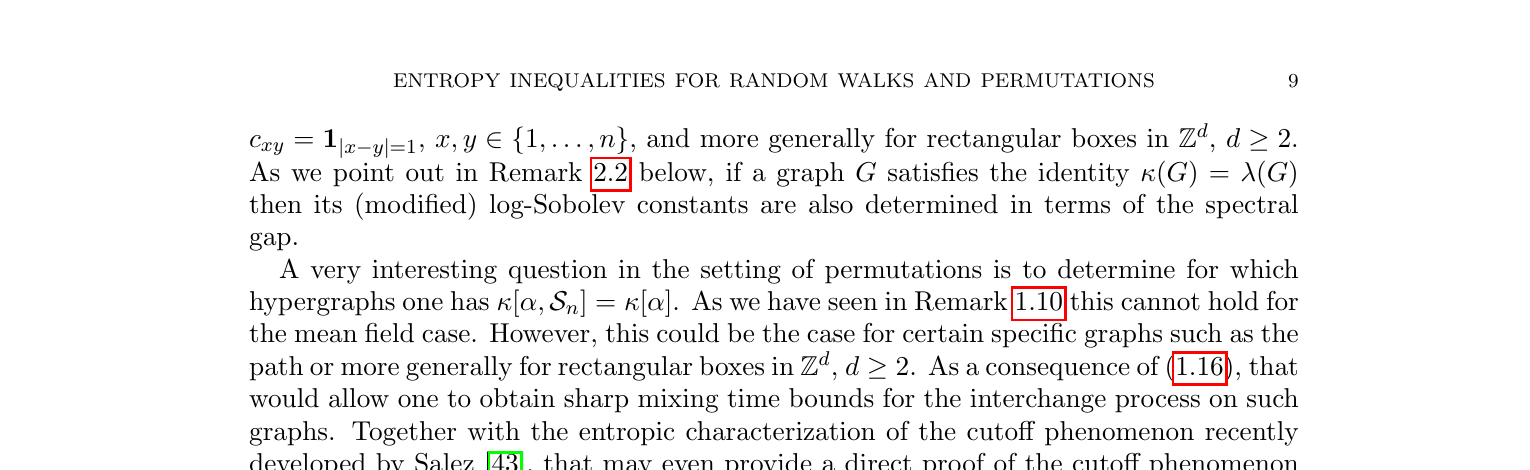
\includegraphics[width=\textwidth]{figures/open_problem_crop_page9.png}
\end{center}

The result below proves an exact tensorization theorem that resolves the
Boolean-box subfamily \(\{0,1\}^d\), including \(C_4\).  It is a substantial
partial result, not a solution for general paths, cycles, or rectangular
boxes.

\section{Definitions and normalization}

Let \(G=(V,c)\) be a finite weighted undirected graph, so
\(c_{xy}=c_{yx}\geq0\) and \(c_{xx}=0\).  Write \(\mu\) for the uniform
probability measure on \(V\).  For \(f:V\to[0,\infty)\), define
\[
  \Ent_\mu(f)
  =\mu[f\log f]-\mu[f]\log\mu[f]
\]
with the convention \(0\log0=0\).  For \(a,b\geq0\), put
\[
 \operatorname{ent}(a,b)
 =\frac a2\log\frac{2a}{a+b}
  +\frac b2\log\frac{2b}{a+b}.
\]
This is the entropy of the two-point function \((a,b)\) under the uniform
measure.  In the normalization of the source, the graph entropy energy is
\[
  \EE_G(f)
  =\frac{2}{|V|}\sum_{x,y\in V}c_{xy}
       \operatorname{ent}(f(x),f(y)),
\]
and
\[
  \ka(G)
  =\inf_{\substack{f\geq0\\ \Ent_\mu(f)>0}}
       \frac{\EE_G(f)}{\Ent_\mu(f)}.
\]

For another weighted graph \(H=(W,d)\), the Cartesian product has vertex
set \(V\times W\) and conductances
\[
 q_{(x,u),(y,v)}
 =c_{xy}\mathbf 1_{\{u=v\}}
  +d_{uv}\mathbf 1_{\{x=y\}}.
\]
All measures below are uniform.

\section{Proof intuition}

There are two independent facts.  First, entropy of a function of two
coordinates is no larger than the average entropy seen along the first
coordinate plus the average entropy seen along the second.  Second, every
edge of a Cartesian product changes exactly one coordinate, so its graph
entropy energy is \emph{exactly} the sum of those same two averaged fiber
energies.  Applying the best factor inequality on each fiber therefore gives
the lower bound for the product constant.  A function depending on only one
coordinate recovers the corresponding factor quotient, giving the matching
upper bound.

\section{Entropy tensorization}

\begin{lemma}[Two-coordinate entropy tensorization]
Let \(\mu,\nu\) be probability measures on finite sets \(V,W\).  For every
\(F:V\times W\to[0,\infty)\),
\[
 \Ent_{\mu\otimes\nu}(F)
 \leq
 \int_W \Ent_\mu(F(\,\cdot\,,u))\,d\nu(u)
 +\int_V \Ent_\nu(F(x,\,\cdot\,))\,d\mu(x).
\]
\end{lemma}

\begin{proof}
Set \(h(u)=\int_V F(x,u)\,d\mu(x)\).  Expanding the definitions gives the
entropy chain rule
\[
 \Ent_{\mu\otimes\nu}(F)
 =
 \int_W\Ent_\mu(F(\,\cdot\,,u))\,d\nu(u)
 +\Ent_\nu(h).
\]
The functional \(g\mapsto\Ent_\nu(g)\) is convex on the nonnegative cone.
Indeed, this is the log-sum inequality (and the boundary follows by
continuity).  Since \(h=\int_V F(x,\,\cdot\,)\,d\mu(x)\), Jensen's inequality
therefore yields
\[
  \Ent_\nu(h)
  \leq\int_V\Ent_\nu(F(x,\,\cdot\,))\,d\mu(x).
\]
Combining the two displays proves the assertion.
\end{proof}

\section{Exact Cartesian-product formula}

\begin{theorem}
For any finite weighted graphs \(G\) and \(H\),
\[
  \boxed{\ \ka(G\BoxProd H)=\min\{\ka(G),\ka(H)\}\ }.
\]
\end{theorem}

\begin{proof}
Let \(n=|V|\), \(m=|W|\), and write \(F^u(x)=F(x,u)\) and
\(F_x(u)=F(x,u)\).  Splitting the ordered edge sum according to which
coordinate changes gives the exact identity
\begin{equation}\label{eq:energy-decomposition}
 \EE_{G\BoxProd H}(F)
 =\frac1m\sum_{u\in W}\EE_G(F^u)
  +\frac1n\sum_{x\in V}\EE_H(F_x).
\end{equation}
For example, the first term on the right is
\[
 \frac1m\sum_u\frac2n\sum_{x,y}c_{xy}
       \operatorname{ent}(F(x,u),F(y,u))
 =\frac{2}{nm}\sum_{u,x,y}c_{xy}
       \operatorname{ent}(F(x,u),F(y,u)),
\]
which is precisely the first-coordinate contribution to the product
energy.  The second term is identical in the other coordinate.

Put \(k=\min\{\ka(G),\ka(H)\}\).  Apply the defining factor inequalities
to every fiber in \eqref{eq:energy-decomposition}, and then use the preceding
lemma:
\begin{align*}
 \EE_{G\BoxProd H}(F)
 &\geq
 k\left\{\frac1m\sum_u\Ent_\mu(F^u)
 +\frac1n\sum_x\Ent_\nu(F_x)\right\}\\
 &\geq k\,\Ent_{\mu\otimes\nu}(F).
\end{align*}
Thus \(\ka(G\BoxProd H)\geq k\).

Conversely, take \(F(x,u)=f(x)\).  Both its global entropy and its product
energy equal the corresponding quantities for \(f\) on \(G\); the
\(H\)-coordinate energy vanishes.  Taking the infimum over \(f\) gives
\(\ka(G\BoxProd H)\leq\ka(G)\).  Functions of \(u\) alone similarly give
\(\ka(G\BoxProd H)\leq\ka(H)\), proving equality.
\end{proof}

\begin{remark}[Spectral gap]
The product Laplacian is the tensor sum
\[
  L_{G\BoxProd H}=L_G\otimes I+I\otimes L_H.
\]
Its eigenvalues are all sums of a factor eigenvalue from \(G\) and one from
\(H\).  Hence
\[
  \la(G\BoxProd H)=\min\{\la(G),\la(H)\}.
\]
It follows immediately that if \(\ka=\la\) holds for both factors, then it
holds for their Cartesian product.
\end{remark}

\section{Weighted Boolean cubes}

\begin{lemma}
For the two-point graph \(K_2(w)\) whose sole edge has conductance \(w>0\),
\[
  \ka(K_2(w))=\la(K_2(w))=2w.
\]
\end{lemma}

\begin{proof}
For \(f=(a,b)\), global entropy is
\(\operatorname{ent}(a,b)\).  The ordered edge sum contains the edge in both
directions, while the prefactor \(2/|V|\) equals one.  Therefore
\[
  \EE_{K_2(w)}(f)=2w\,\operatorname{ent}(a,b)
                 =2w\,\Ent(f).
\]
Thus \(\ka(K_2(w))=2w\).  The weighted Laplacian matrix
\[
  \begin{pmatrix}w&-w\\-w&w\end{pmatrix}
\]
has eigenvalues \(0\) and \(2w\), proving the spectral statement.
\end{proof}

\begin{corollary}
Let
\[
 Q_d(w_1,\ldots,w_d)
 =K_2(w_1)\BoxProd\cdots\BoxProd K_2(w_d),
 \qquad w_i>0.
\]
Then
\[
 \boxed{\ 
 \ka\bigl(Q_d(w_1,\ldots,w_d)\bigr)
 =\la\bigl(Q_d(w_1,\ldots,w_d)\bigr)
 =2\min_{1\leq i\leq d}w_i\ }.
\]
In particular, all unweighted Boolean boxes have
\(\ka=\la=2\), and \(C_4=K_2\BoxProd K_2\) satisfies the cycle conjecture.
\end{corollary}

\begin{proof}
Iterate the entropy-constant product theorem and the spectral-gap product
formula, using the preceding two-point computation in each coordinate.
\end{proof}

\section{Independent checks and novelty scope}

A deterministic verifier included with this packet checks:
\begin{enumerate}[leftmargin=2em]
\item entropy tensorization on 2,000 random positive two-factor arrays;
\item the exact energy decomposition on the corresponding random weighted
graph products;
\item the quotient \(2w\) for 100 weighted two-point instances; and
\item the claimed inequality on 1,200 weighted cubes of dimensions one
through six.
\end{enumerate}
These computations are checks of normalization and implementation, not a
substitute for the proof.

The run's local indexes were searched by identifier, title, and the core
product/tensorization terminology.  A bounded web search found the source
paper and general background, but no exact statement of the displayed
product formula or weighted-cube corollary.  The theorem may nevertheless be
folklore; the novelty claim is therefore deliberately modest and requires
expert review.

An exploratory multi-start minimization of the exact quotient on paths and
cycles through ten vertices found no credible strict counterexample.  That
experiment is not used in the proof.  The cases of longer paths, longer
cycles, and boxes having any side length greater than two remain outside this
packet.

\section*{Reference}

A. Bristiel and P. Caputo, \emph{Entropy inequalities for random walks and
permutations}, Ann. Inst. Henri Poincar\'e Probab. Stat.
\textbf{59} (2023), no.~4, 2280--2310; arXiv:2109.06009.

\section*{Human-review recommendation}

Review as a likely valid partial result.  The high-value checks are:
(i) equation~\eqref{eq:energy-decomposition} under the source normalization;
(ii) convexity of entropy in the tensorization lemma; and (iii) the factor
\(2w\) in the two-point graph.

\end{document}
